\section{Experimental setup for Pockels effect}
\subsection{Setup}
\label{sec:setup_pockels}
The experimental setup is consists of the beam bath with the Pockels Cell, 
two polarizators and a photodiode as well as the signal generating and 
analysing electronics. The beam is produced by a HeNe laser operating in 
the red part of the visualspectrum and guaranteeing monocromatic light 
at 632.8nm in air~\cite{versuchsanleitung}. 

A block diagram of the setup is given in figure \ref{fig:setup_block}, 
the actual instruments are shown in the photo \ref{fig:setup_photo}. 

\begin{figure}
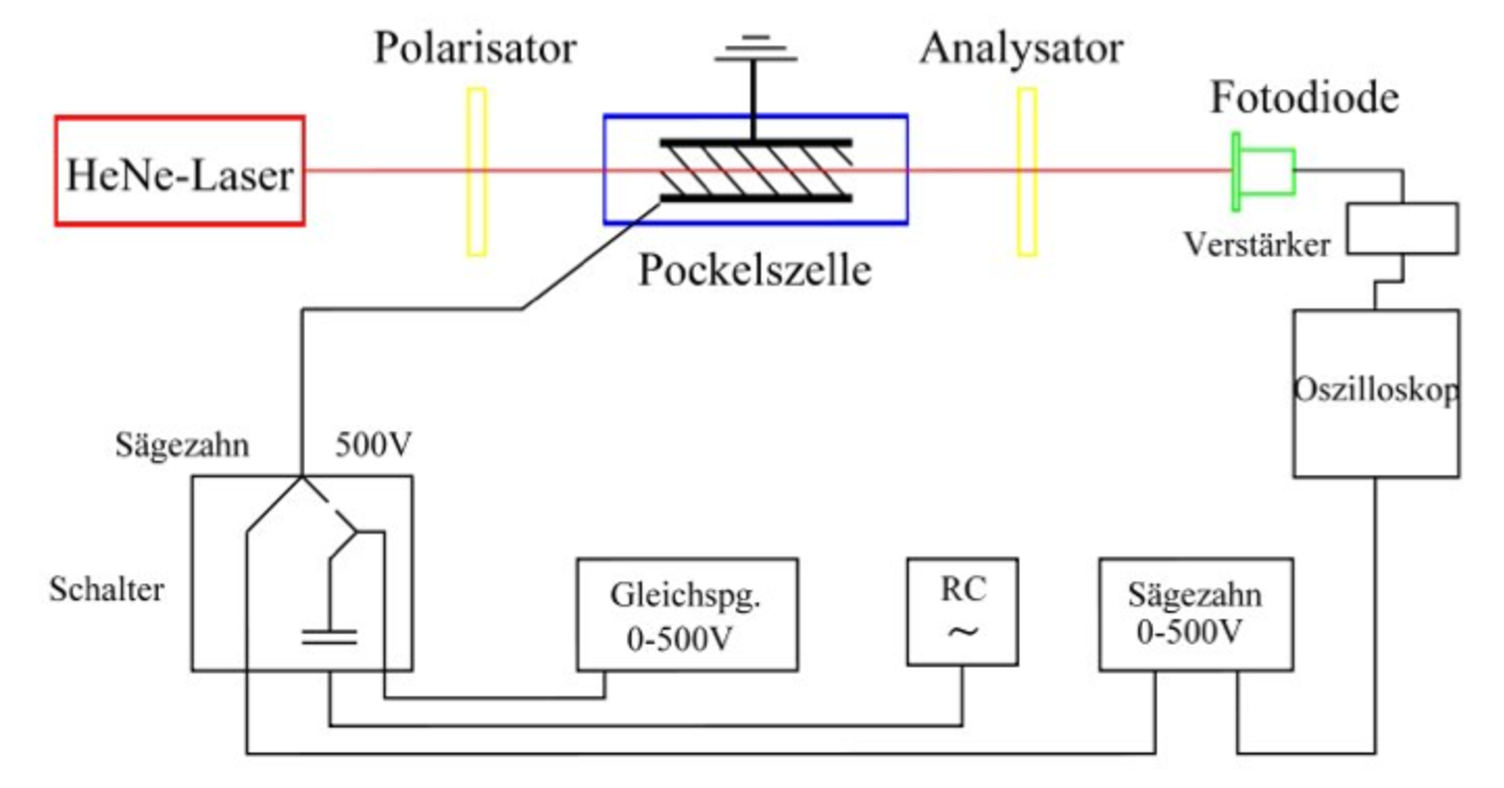
\includegraphics[width=\pltw]{figures/setup_block.pdf}
\caption{
    Block diagram of the experimental setup for measuring the 
    Pockels effect, 
    from~\cite{versuchsanleitung}.
    }
\label{fig:setup_block}
\end{figure}

\begin{figure}
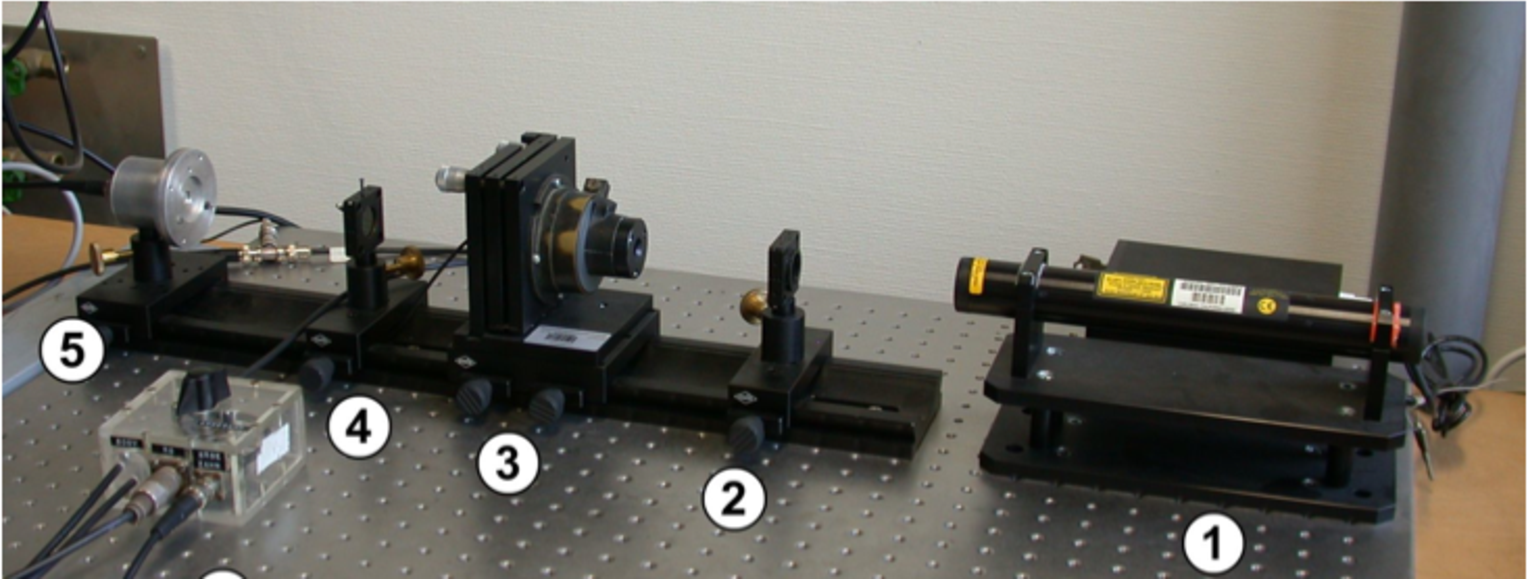
\includegraphics[width=\textwidth]{figures/setup_photo.pdf}
\caption{
    Photo of the experimental setup for measuring the 
    Pockels effect with the following devices:
    1) He-Ne-Laser, 2) polarisator, 3) Pockels Cell, 
    4) analysator, 5) photodiode;
    modified from~\cite{versuchsanleitung}.
    }
\label{fig:setup_photo}
\end{figure}

The Pockels Cell consists of four ADP crystals aligned in the beam path, 
as shown in figure \ref{fig:pockels_cell_path}.

\begin{figure}
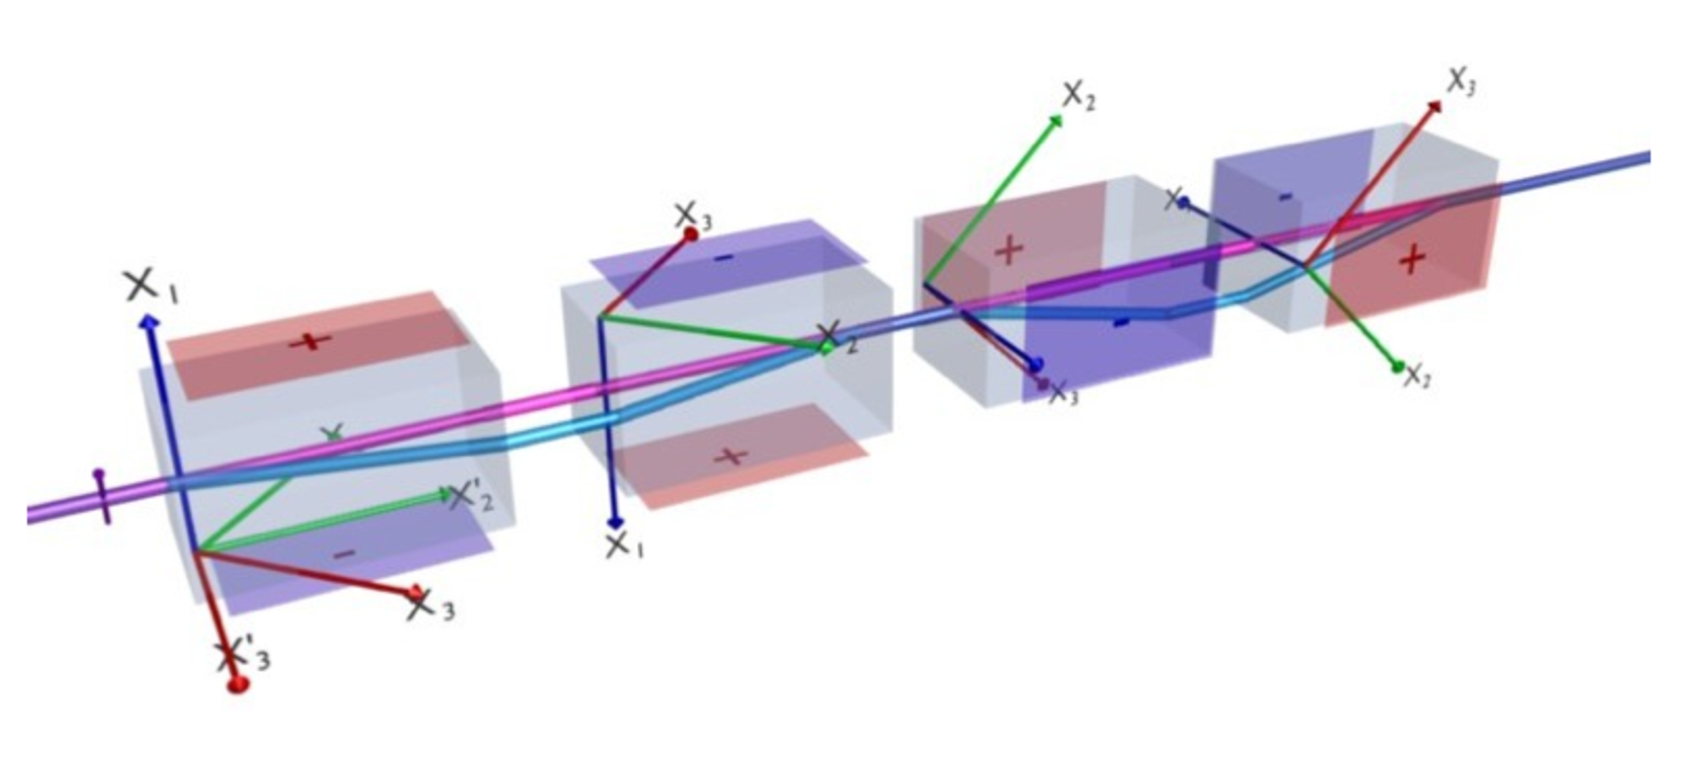
\includegraphics[width=\textwidth]{figures/pockels_cell_path.pdf}
\caption{
    Alignment of crystals of the Pockels Cell. One can the the different 
    rotations of the crystals and the applied electric fields 
    relative to each other, cancelling the separation of beams and 
    natural double refraction. The birefringence of 
    the beam path is shown schematically with the blue and violet beam. 
    From~\cite{versuchsanleitung}.
    }
\label{fig:pockels_cell_path}
\end{figure}

The eletric fields are applied by condensators with the plates 
orientated perpendicular to the $x_1$ axis of the crystal in 
it's principle dieletric axes system, which implies, that the 
$x_3$ axis of fourfold rotoinversion is parallel to the condensator 
plates. As elaborated in the theoretical section, this 
setup corresponds to the \emph{transverse Pockels effect}. 
All crystals are prepared in the $45\Deg$-Y-cut relative to the crystal 
lattice. The light thus enters in the direction of the line 
bisecting the $x_3$ and $x_2$ axis of the crystal. This direction 
is named $x_2'$. 
In order to annul the separation of the arising two beams, 
the first two and the second two crystals and their condensators 
are rotated by $180\Deg$ one to another. The second pair is 
further rotated by $90\Deg$ and has it's electric field inverted, 
such that the naturally arising birefringence is cancelled. 

The parameters of the used Pockels cell are shown in 
table \ref{tab:pockels_technical}.

\begin{table}[htdp]
    \begin{tabular}{|p{0.61\textwidth}|p{0.37\textwidth}|}
        \hline
        Number of crystals & 4 \\
        Crystal cut & $45\Deg$-Y-cut \\
        Wavelenght of HeNe Laser & 632.8 nm \\
        Thickness of crystall & $d = 2.4$ mm \\
        Refractive index in $x_1$ and $x_2$ direction & $n_1 = 1.522$  \\
        Refractive index in $x_3$ direction & $n_3 = 1.477$  \\
        Electro-optic coefficient & $r_{41} = 23.4$ pm / V @ $ 20\Deg$ C \\
        \hline
    \end{tabular}
\caption{
    Technical data of the ADP-Pockels Cell,
    taken from~\cite{versuchsanleitung}.
    }
\label{tab:pockels_technical}
\end{table}

\begin{samepage}
The electronical devices for generating and analysing the signal are 
\begin{itemize}
    \item
    function generator: Voltcraft MX 2020;
    \item
    saw tooth operator: self-built (M 1657);
    \item
    Pockels Cell: Leysop EM 200 A;
    \item
    oscilloscope: Hameg HM 1507.
\end{itemize}
\end{samepage}


\subsection{Methods of determining $\Ula$}
In order to determine $\Ula$, we measure the intensity of the laser 
passing a linear polarization filter, the Pockels Cell and a second filter 
in perpendicular orientation, which acts as an analysator. 
As derived in the theoretical section~\ref{sec:application_cell},
the Pockels effect is expected to introduce a phase difference 
of $\pi$ for the two perpendicularly polarized components of the 
incoming wave. We thus expect a maximum of intensity for the applied 
voltage $\Ula$ and a minimum for $U = 0$ and $U = 2\Ula$. 
We apply the following two methods to find $\Ula$ experimentally:
\subsubsection{Saw tooth}
The voltage follows a saw tooth signal, increasing linearly from 0 V up to 500 V 
at a frequency of ca. 30 Hz. An oscilloscope records the intensity measured 
at a photodiode in phase with the saw tooth signal, which is deamplified 
by a resitor by a factor of approximately 100. 
We can measure the distance in time between minimum and maximum of the signal 
and then linearly extrapolate the corrisponding input voltage at the maximum.
\subsubsection{Modulated direct current}
Here, we use a direct current $U_\mathrm{DC} \in (0, 300)$ V modulated by a 
sine $U_\mathrm{AC}$ of amplitude $40 \ \mathrm{V_{pp}}$. 
For $U_\mathrm{DC} \ll \Ula$, an AC-coupled 
oscilloscope is expected to show a response following the sine. However, for 
$U_\mathrm{DC} = \Ula$, each time $U_\mathrm{AC} = 0$, the response shows a maxima. 
Accordingly, we expect a frequency doubling in the intensity signal. 
We thus try to find $\Ula$ by measuring $U_\mathrm{DC}$ once 
frequency doubling occurs. 
We take several measurements close to the frequency doubling
and obtain the values of the input signal 
$U_\mathrm{in} \propto U_\mathrm{AC}$, 
and the response signal $U_\mathrm{out}$. 
In order to find the point of frequency doubling we analyse 
the amplitudes of the power spectral density 
\begin{equation}
    \mathrm{psd}(\nu) \mathrm{d}\nu \propto |\mathrm{FFT}[U(t)]|^2
\end{equation}
at the frequencies 
$\nu_1$ and $\nu_2 = 2\nu_1$, where $\nu_1$ is the frequency 
of the $U_\mathrm{AC}$ input signal. 
The fast fourier transformation (FFT) is computing the discrete 
Fourier transform (DFT) of the response signal $U_\mathrm{out}(t)$. 
The used algorithm is the function 'numpy.fft',
which is part of the python library 'SciPy'~\ref{scipy}. 
The window for the FFT is defined by the first and the last minimum 
of the input signal $U_\mathrm{in}$, 
which is searched numerically by finding the absolute minimum of the array 
$U_\mathrm{in}$ restricted to $t \in (1, 1.5)$ ms and $t \in (8.5, 9.5)$ ms, 
respectively. 

\subsection{Properties of He-Ne-Laser}
In this experimental setup we use a helium-neon laser, which is one of the most popular lasers.
The inherent gain medium consists of a 10-1 ratio mixture of helium and neon 
at a pressure of 10mbar. The laser
was developed in 1961 as first \textbf{continuous wave}-laser. It has been used since then to
study general properties of lasers and of coherent light in general, which originates from
the neonatoms being stimulated by the helium. Nowadays helium-neon lasers are more and more
replaced and substituted by the more compact and inexpensive laser diode.
The functional principle is as following: A external induced discharge causes the helium atomes
to shift into a higher, persistent energy level. From this time the neonatomes can be stimulated
continuosly with a high efficiency and cause thus an inversion of the higher energy levels.
Without helium we would not see the higher excited states. The pump source of the laser
is in general realized by a high voltage electrical discharge coming from an anode and
cathode with the gas in between, within the tube. Since the intensity is connected to the
pressure it is possible to increase the length of the tube in order to amplify the beam, which
has other disadvantages, for instance the appeareance of other unwanted lines.
The electromagnetic field $E(\rho = \sqrt{x^2 + y^2}, y)$ with Amplitude $E_0$ 
generated by the laser can be treated approximately as a gaussian
beam~\cite{boyd2003nonlinear}, which follows the following equation:
\begin{equation}
    E(\rho,z) = \frac{E_0 w_0}{w(z)} \mathrm{Exp} \left[  
        \frac{ik\rho^2}{2R(z)} + i\phi(x) - \left( \frac{\rho}{w(z)} \right)^2    \right]
\end{equation}
Where we introduced the 1/e radious of the field distribution
\begin{align}
    w(z) = w_0 \sqrt{ 1 +\left (\frac{\lambda z}{\pi w_0^2} \right )^2}
\end{align}
and the radius of the curvature of the optical wavefront with
\begin{equation}
    R(z) = z \left[ 1 + \left( \frac{\pi w_0^2}{\lambda z} \right)^2 \right]
\end{equation}
and the spatial variation of the phase of the wave
\begin{equation}
    \phi(z) = - \mathrm{Arctan} \left( \frac{\lambda z}{\pi w_0^2} \right) 
\end{equation}

\begin{SCfigure}
    \begin{centering}
        \caption{The inversion of the helium-neon laser~\cite{christian2003gerthsen}. 
            As result of the electronscattering the
    heliumatoms are shifted into persistent states, from which they transmit their energy by
    interaction to the neon. The highest laser activity is realized
    through the shift of 3s to 2p states ($633nm$) but other lines are possible as well,
    for instance from 3s to 3p ($3.39 \mu m$) or from 2s to 2p ($1.15\mu m$). The mechanism
    producing this population inversion and the light amplification in the plasma is due
    to the inelastic scattering of the electrons with ground state helium atoms in the gas
    mixture.}
        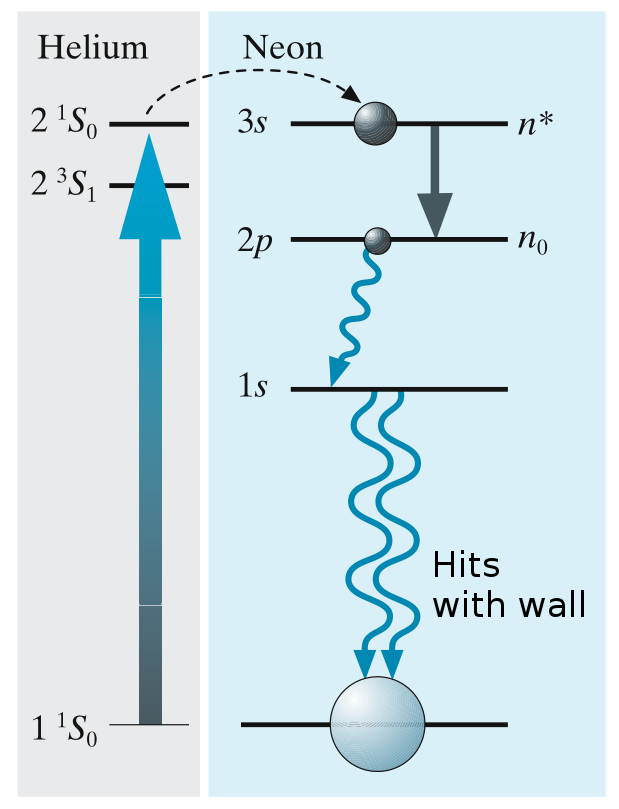
\includegraphics[width=8cm]{figures/helium-neon-laser}
        \label{fig:integral}
    \end{centering}
\end{SCfigure}

\begin{SCfigure}
    \begin{centering}
    \caption{Different aspects of the gaussian nature of the laser beam~\cite{boyd2003nonlinear}.
        (a) Field amplitude distribution of a gaussian laser beam. (b) Variation of the beam
        radius $w$ and wavefront radius of curvature R with position $z$.
        (c) Relation between the beam waist radius and the confocal parameter $b$. }
        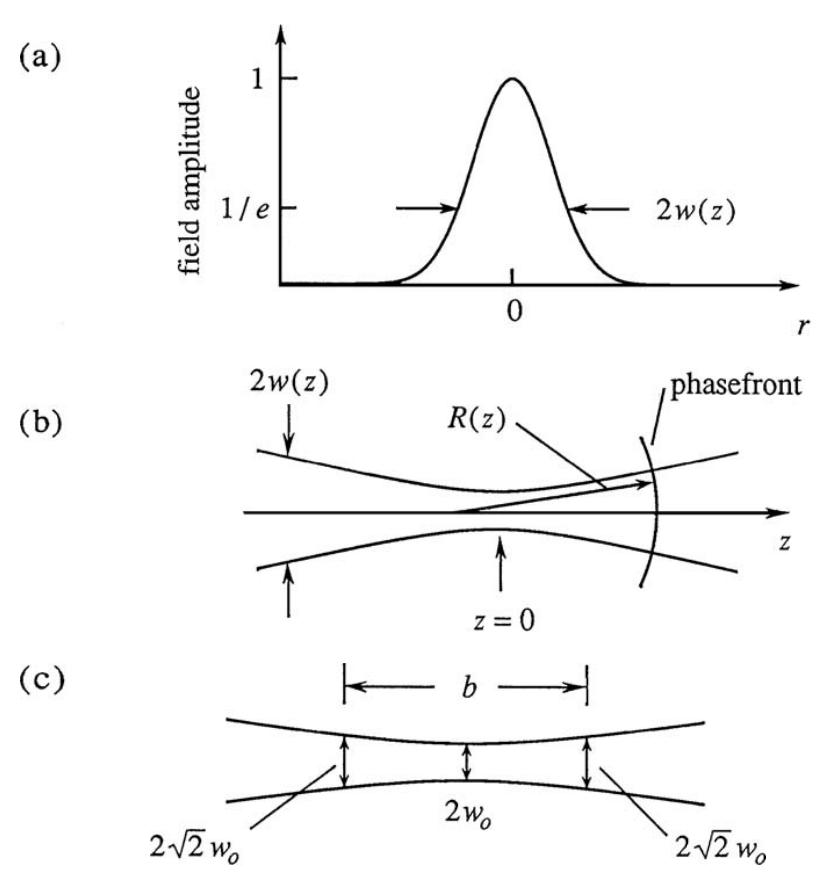
\includegraphics[width=10cm]{figures/gaussian}
        \label{fig:integral}
    \end{centering}
\end{SCfigure}
The beam waist radius $w_{0}$ can be calculated in terms of the Power $P$, which we can retrieve
by integrating:
\begin{equation}
    P = n \epsilon_0 c \pi w_0^2 |E_0|^2
\end{equation}
Unfortunatelly in our experimental setup it was neither possible to modificate the position of
the laser nor to adjust the setup in a way that we could have measured the specifications of 
the laser, so it is not possible for us to include dispersion or diffraction phenomena originating
from the gaussian nature of the beam into our considerations regarding to the analysis of the 
experiment. We added some notes in the chapter~\ref{sec:laser} ``
Further investigations regarding the laser''.

